%%%%%%%%Bilecik �eyh Edebali �niversitesi M�hendsilik Fak�ltesi%%%%
%%%%%%%%%%%Bilgisayar M�hendisli�i Proje I-II �al��mas�%%%%%%%%%%%%
%%%%%%%%%%%%%%%%%%%%%%LaTeX Class%%%%%%%%%%%%%%%%%%%%%%%%%%%%%%%%%%
\documentclass{BUP}
%%%%%%%%%%%%%%%%%%%%%%%%%%%%%%%%%%%%%%%%%%%%%%%%%%%%%%%%%%%%%%%%%%%%%%%%%%%
\begin{document}
\shorthandoff{=}%grafik komutlar�nda babelden kaynaklanan hatay� engeller.
%%%%%%%%%%%%%Proje I-II �al��malar�n�n B�l�mleri%%%%%%%%%%%%%%%%%%%%%%%%%%%
\thispagestyle{empty} %Bu sayfaya sayfa numaralar� yaz�lmaz
\begin{figure}[H]
\centering

\includegraphics[scale=0.2]{logomuz}
%Bu komutla resim dosyam�z� y�kl�yoruz.
\end{figure}
%sa�a 4 sol 2 a�a�� yukar� 3%
\begin{center}
\textbf{T.C.}\\
\textbf{B�LEC�K �EYH EDEBAL� �N�VERS�TES�}\\
\textbf{M�HEND�SL�K FAK�LTES�}

\textbf{B�LG�SAYAR M�HEND�SL��� B�L�M�}
\end{center}

\vspace*{4cm}%bir miktar bo�luk b�rakmak i�in
\begin{center}
\textbf{NODEJS �LE SOHBET UYGULAMASI}

\textbf{Mustafa YILDIRIM}

\textbf{B�LG�SAYAR M�HEND�SL��� TASARIM �ALI�MASI I}
\end{center}

\vspace*{\fill}
\begin{center}
\textbf{DANI�MANI : Murat �ZALP}

\textbf{B�LEC�K}\\ 
\textbf{\today}
\end{center}

\thispagestyle{empty} %Bu sayfaya sayfa numaralar� yaz�lmaz

\begin{figure}[H]
\centering

\includegraphics[scale=0.2]{logomuz}
%Bu komutla resim dosyam�z� y�kl�yoruz.
\end{figure}
%sa� 4 sol 2 a�a�� yukar� 3%
\begin{center}
\textbf{T.C.}\\
\textbf{B�LEC�K �EYH EDEBAL� �N�VERS�TES�}\\
\textbf{M�HEND�SL�K FAK�LTES�}

\textbf{B�LG�SAYAR M�HEND�SL��� B�L�M�}
\end{center}

\vspace*{4cm}%bir miktar bo�luk b�rakmak i�in
\begin{center}
\textbf{NODEJS �LE SOHBET UYGULAMASI}

\textbf{Mustafa YILDIRIM}

\textbf{B�LG�SAYAR M�HEND�SL��� TASARIM �ALI�MASI I}
\end{center}

\vspace*{\fill}
\begin{center}
\textbf{DANI�MANI : Murat �ZALP}

\textbf{B�LEC�K}\\ 
\textbf{\today}
\end{center}

\pagenumbering{roman}%romen rakamlar� kullan�lmaya ba�lan�yor.
\setcounter{page}{2}% sayfa numaras�n� ii'den ba�lat�l�yor.
\centerline{\bf �ZET}
\addcontentsline{toc}{section}{�ZET}
\begin{center}
\textbf{Projenin Amac�}
\end{center} 
 \mbox{	Web �zerinde responsive olarak �al��acak mesajla�ma uygulamas� yapmak.}

\begin{center}
\textbf{Projenin Kapsam�}
\end{center}
 \mbox{	Proje kapsam�nda front-end ba�lamlar�m� bir arada tutmak i�in bower compenents kullanarak}
 \mbox{angular dosyalar�m� burada tuttum. Back-end yap�land�rmalar�m� Node.JS ile ger�ekle�tirip veri}
 \mbox{taban�nda NoSQL yap�s�n� tercih edip MongoDB kulland�m bunlara ek olarak ger�ek zamanl�}
 \mbox{i�lerimi ger�ekle�tirebilmek i�in Ajax yerine Socket.Io ile i�lemlerimi ger�ekle�tirdim son olarak}
 \mbox{Redis ile t�m session bilgilerini, mesajlar�, odalar� ve aktif olan kullan�c�lar� tuttum. }
 \mbox{}

\begin{center}
\textbf{Sonu�lar}
\end{center}
 \mbox{	Projenin kapsam�na uyularak ilerlenmi� ve gerekli t�m yap�land�rmalar yap�larak proje digital }
 \mbox{ocean ile canl� ortama ta��nm��t�r.}
%%%%%%%%%%%%%%%%%%%%%%%%%%%%%%%%%%%%%%%ABSTRACT%%%%%%%%%%%%%%%%%%%%%%%%%%%%%%%%%%%%%%%%%%
\newpage
\centerline{\bf ABSTRACT}
\addcontentsline{toc}{section}{ABSTRACT}
\begin{center}
\textbf{Project Objective}
\end{center}

 \mbox{
	Do the messaging app that will run responsibly on the web.}

\begin{center}
\textbf{Scope of Project}
\end{center}
 \mbox{	I kept my angular files using bower compenents to keep my frontend contexts together. I have}
 \mbox{implemented backend configurations with Node.JS and I have chosen the NoSQL structure in}
 \mbox{the database. I used MongoDB to perform real-time tasks in addition to Ajax instead of Socket.Io}
 \mbox{and finally  I used all the session information, messages, chambers and active users with Redis.}

\begin{center}
\textbf{Results}
\end{center}
 \mbox{	The project was carried out in accordance with the scope of the project and all the necessary}
 \mbox{configurations were made and the project was carried to the live environment with the digital}
 \mbox{ ocean.}
\addcontentsline{toc}{section}{TE�EKK�R}
\section*{TE�EKK�R}
Bu projenin ba��ndan sonuna kadar haz�rlanmas�nda  eme�i bulunan ve 
beni bu konuya y�nlendiren sayg�de�er hocam ve dan��man�m 
Say�n Murat �ZALP'e t�m katk�lar�ndan ve hi� 
eksiltmedi�i deste�inden dolay� te�ekk�r ederim.
\vspace{2cm}

\begin{flushright}
\textbf{Mustafa YILDIRIM}

\today
\end{flushright}
\tableofcontents%bu komutun oldu�u yerde i�indekiler olu�turulur.
%\textbf{\centerline{\bf S�MGE L�STES�}}
\addcontentsline{toc}{section}{S�MGE L�STES�}

\renewcommand*\listfigurename{\centerline{\bf\normalsize �EK�L L�STES�}}
\listoffigures%bu komutun oldu�u yerde �ekiller listesi olu�turulur
\addcontentsline{toc}{section}{�EK�L L�STES�}
%\renewcommand*\listtablename{\centerline{\bf\normalsize TABLO L�STES�}}
\listoftables%bu komutun oldu�u yerde tablolar listesi olu�turulur
\addcontentsline{toc}{section}{TABLO L�STES�}
\pagenumbering{arabic}%Sayfa numaralamas�n� arap rakamlar�yla yapar.
\setcounter{page}{1}%sayfa numaras�n� 1'den ba�lat�r.
\section{G�R��}
\subsection{Projenin Genel Hatlar�yla Anlat�m�}
	Bu alanda projeyi �zet olarak tekrardan anlatmak istiyorum. �lk olarak projeyi anlatay�m. Asl�nda bak�ld��� zaman tamamiyle bir mesajla�ma uygulamas�d�r ama neden b�yle bir uygulama yazd�m. Kulland���m teknolojiler neler bunlar hakk�nda biraz bilgi vereyim. Yazd���m projede socket.io ile gelen mesajlar�, oda ekleme i�lemi ve aktif olan kullan�c�lar� an�nda g�rmemize imkan sa�lamaktad�r. Peki nedir bu Socket.Io ve neden Ajax kullanmad�m da Socket.Io kulland�m. Durumu ��yle anlatabilice�imi umuyorum. E�er ileti�imimiz tek bir y�nde ise �rne�in m��teri her zaman sunucuyla ileti�imi ba�latan ki�iyse AJAX'� kullanmak daha verimli olacakt�r. ��nk� daha h�zl� uygulayabiliriz ama burada sunucu ile m��teri aras�nda her iki y�nde ak�c� bir �ekilde ileti�im kurmam�z gerekti�i i�in Socket.Io se�imi bizim i�in en do�ru se�im olacakt�r ki Socket.Io'nun bir ba�ka b�y�k avantaj�, t�m m��terilerle belirli bir anda �evrimi�i olarak ileti�im kurabilmemiz. �kisi aras�nda kar��la�t�rma yapt���m�zda ve yapaca��m�z i�in mesajla�ma oldu�unu d���n�rsek en mant�kl� tercihin Socket.Io oldu�u olduk�a a�ikard�r.
	Tamam Socket.Io'yu kulland�k projeyi geli�tiriyoruz peki bundan sonras� nas�l olacak burada yapmam�z gereken iki olay var verilerin kaydedilmesi ve Socket.Io ile tuttu�umuz verilerin frond-end de g�sterilmesi. �nce frond-end de g�sterilmesi �zerine dural�m. Burada bize client ba�lant�s� olan ve frond-end i�in kullanabilece�imiz frameworklerden birini se�ersek i�lerimiz bir hayli kolay olacak ve i�leri o kadar h�zl� ilerletece�iz ben bunun i�in Angular'� tercih ettim Vue.Js, React veya di�erleri de se�ilebilirdi. Benim Angular'� se�memin nedenleri aras�nda frameworkler aras�nda en olgun olan� olmas�, katk�da bulunanlar a��s�ndan iyi bir deste�inin olmas� ve en �nemlisi eksiksiz bir paket olu�udur. �imdi frond-end yap�land�rmam�z� da halletti�imize g�re uygulamam�z�n veri taban� i�in kulland���m iki veri taban�n� anlatmaya ba�lay�m. Bu veri tabanlar�ndan birisi sadece kullan�c�lar�m�n Google Id gibi giri� bilgilerini tutmaktad�r. Bu NoSQL olan MongoDB ile yap�lmaktad�r. Bunun haricinde t�m mesajlar�n tutuldu�u, online olan kullan�c�lar�n tutuldu�u, kullan�c�lar�n session bilgileirinin tutuldu�u ve son olarak eklenen odalar�n tutuldu�u Redis'dir..
	Bu yap�lar�n hepsi ve kulland���m paketler ileride ayr�nt�l� bir bi�imde anlat�lacakt�r.
	Yani sonu� olarak burada yapt���m�z i� �n tarafta Framework olarak Angular kullanarak, html yerine pug tercihi yapt�m sayfalar� yazarken bununda birka� nedeni vard�r ileride anlataca��m arka tarafta Node.js'in paketi olan Socket.Io ile i�lemleri y�r�tt�m ve redis ile verilerimi tutarak bir mesajla�ma uygulamas� yapt�m.
	\subsection{Neden bu projeyi se�tim}
	Bu projeyi se�memin en b�y�k etkeni proje hocamd�r. Bana daha �nce yapt���m projeden farkl� bir proje olmas� ve CV'ne yazaca��n farkl� �eyler olsun diye birka� kere tavsiye verdi�inden dolay� ve php ile node.js alan�ndaki i�lerin �lkemizde �ok yak�n d�� �lkelerde ise node.js'in �nde olmas�n�ndan �t�r� b�yle bir proje yapmay� tercih ettim neticede bu projedeki temel amac�m Node.Js ��renmek ve CV'me yaz�labilecek birka� sat�r eklemekti.
	\subsection{Bu proje ile hedeflenen ve faydalar�}
	Bu proje ile Socket.Io ile gelen verilerin anl�k olarak i�lenmesi ve Redis'e kaydedilmesi hedeflenmi�tir. Bunlarda Socket.Io mesajla�ma uygulamalar� i�in bi�ilmi� kaftand�r olduk�a h�zl� bir �ekilde kullan�c�lar�n haberle�melerini sa�lamaktad�r. Di�er taraftan Redis en basit haliyle, key-value �eklinde tasarlanm�� bir NoSQL veritaban�d�r ve �ok h�zl�d�r bunun nedenide Memcached gibi verileri HDD yazmadan RAM �zerinde tuttu�undand�r. Bu ikiliyi birle�tirdi�imizde ise bize olduk�a h�zl� bir mesajla�ma platformu haz�rlanm�� oluyor.
	\subsection{Kullan�lan Bile�enler}
	Bu alanda kullan�lan bile�enler k�sa bir �ekilde anlat�lacak olup daha ayr�nt�l� bilgi i�in bir sonraki b�l�me bakman�z proje sorumlusu taraf�ndan �nerilmektedir.
	Ba�lad���m�zdan beri hep node.js den bahsetmekteyiz peki biz bu node.js'i hangi dille yaz�yoruz �imdi her�eyi bir s�rayla teker teker ele alal�m.
	\subsubsection{JavaScript}
	JavaScript, yayg�n olarak web taray�c�lar�nda kullan�lmakta olan bir betik dilidir. JavaScript ile yaz�lan istemci taraf� betikler sayesinde taray�c�n�n kullan�c�yla etkile�imde bulunmas�, taray�c�n�n kontrol edilmesi, asenkron bir �ekilde sunucu ile ileti�ime ge�ilmesi ve web sayfas� i�eri�inin de�i�tirilmesi gibi i�levler sa�lan�r. JavaScript, Node.js gibi platformlar sayesinde sunucu taraf�nda da yayg�n olarak kullan�lmaktad�r.

�lk olarak bir Netscape �al��an� olan Brendan Eich taraf�ndan geli�tirilen ve 1997 y�l�ndan beri bir ECMA standard� olan JavaScript, g�n�m�zde Mozilla Vakf� �nc�l���nde �zg�r yaz�l�m toplulu�u taraf�ndan geli�tirilmekte ve bak�m� yap�lmaktad�r.
Web sayfalar�n�n g�r�n�m�n�n m�kemmelle�tirilmesi, i�levselli�inin art�r�lmas� ve dinamik web sayfalar� tasarlanmas� amac�yla JavaScript, HTML kodu i�inde g�m�l� olarak (embedded) kullan�labilir. JavaScript, bir programlama dili disiplini ve �zelliklerine sahiptir.
	\subsubsection{Node.JS}
	Node.js, JavaScript'dir. Web taray�c�lar�na muhta� kalmadan heryerde �al��abilir. Peki ne i�e yarar bir yaz�l�m�n hem arkay�z (back-end) hem �ny�z (front-end) kodlar�n� ayn� dilde yazman�n tek yoludur. G�n�m�zde �o�u uygulama, zaman�n�n �o�unu veritabanlar�na veya Internet'deki �e�itli servislere istek yap�p gelen sonu�lar� beklemekle getiriyorlar. Node.js, yap�s� gere�i asenkrondur. �stekleri paralel olarak yapar. �stekler bittikleri zaman Node'a callback yaparlar. Bu sayede anl�k olarak �ok say�da istek h�zl� bir �ekilde i�lenebilir.
	\subsubsection{Angular}
	Angular javascript tabanl� a��k kaynak kodlu yaz�l�m geli�tiricilerin web, mobil ve masa�st� ortamda kolay uygulama geli�tirmelerini sa�layan bir platformdur. Ayr�ca istemci taraf�nda �al��an yada daha a��k bir ifade ile kullan�c�lar�n g�rebildi�i ve etkile�ebildi�i ortamlarda (web taray�c�lar�nda) �al��an bir framework oldu�u i�in bir Front-End Development prati�idir.
	\subsubsection{MongoDB}
	MongoDB bize kendisini, geli�tirme ve �l�ekleme kolayl��� i�in tasarlanm�� a��k kaynak, belge y�nelimli(document-oriented) veritaban� olarak tan�tmaktad�r. MongoDB'de her kay�t, asl�nda bir d�k�mand�r. D�k�manlar MongoDB'de JSON benzeri Binary JSON(BSN) format�nda saklan�r. BSON belgeleri, saklad�klar� elemanlar�n s�ral� bir listesini i�eren nesnelerdir. Herbir eleman, bir alan ad� ve belirli tipte bir de�erden olu�ur.
	\subsubsection{Redis}
	En basit haliyle Redis, key-value �eklinde tasarlanm�� bir NoSQL veritaban�d�r. Memcached gibi verileri HDD yazmadan Ram �zerinde tutmaya yarayan bir platformdur. Memcahedden farkl� olarak NoSql mant���yla �al��t��� i�in serverin kapansa dahi verilerin kaybolmas�na izin vermez.

\newpage
\section{KULLANILAN TEKNOLOJ�LER}
Bu b�l�mde projede kullan�lan teknolojilerin tamam� ayr�nt�l� bir bi�imde anlat�lacakt�r.
\subsection{Node.Js'e Giri�}
	NodeJS, server-side (sunucu tarafli) uygulamalar geli�tirmek i�in �retilmi� bir teknolojidir. �lk yay�nland��� 2009 tarihinden bug�ne di�er geleneksel sunucu tarafl� uygulama teknolojilerinin aksine, bir�ok alanda farkl� yap�s�yla t�r�n�n �nc�s� olmu�tur.
	\textbf{Ryan Dahl} hen�z 1 sene �nce (2008 y�l�nda) Google'�n Chrome taray�c� i�in geli�tirmi� oldu�u \textbf{v8 engine}'in �zerine olu�turdu�u mimariyle, \textbf{JavaScript} ile \textbf{Back-end} uygulama geli�tirebilece�ini g�stermi�tir. Bu noktada v8'in yap�s� gere�i sadece Web Browser �zerinde JavaScript �al��t�rmak i�in yap�ld���ndan Back-end k�sm�nda dosya i�lemleri gibi bir�ok �zelli�i i�inde bulun\textbf{ma}maktayd�. NodeJS bunun gibi pek �ok ekstra yap�y� ve \textbf{V8}'i extend ederek b�nyesinde bar�nd�rmaktad�r.
	
	V8 engine C++ diliyle geli�tirilmi�tir. Runtime'da JavaScript kodlar�n� makina koduna d�n��t�r�r ve sonras�nda native makina kodunu �al��t�r�r. Hem Node projelerinin hem Chromium projesinin bu kadar performansl� olmas�n�n arkas�nda yatan sebep budur.
	
	NodeJS, \textbf{Single Thread Non-Blocking IO}, Asenkron programlama gibi pek �ok �zelli�i ile �ne ��kmaktad�r.
	
	NodeJS \textbf{Community}'si olduk�a b�y�k olmas�n�n yan�nda Yahoo, Microsoft, LinkedIn, Uber, Paypal gibi pek �ok dev firman�n yaz�l�m sistemleri i�erisinde bir pay edinmesi bu ba�ar�n� g�steren en �nemli kan�tlardan biridir.
	
	As�l amac� Back-end projeler geli�tirmek olmakla birlikte NodeJs, Front-end otomasyonu ve package management gibi yaz�l�mlar�n pek �ok alan�nda �ok y�nl�l��� ile kar��m�za ��kmaktad�r.
	
\subsection{Ecmascript 6 ve NodeJS}
	Bu proje haz�rland��� a�amada Ecmascript 7 ve 8 ��km�� bulunmaktad�r. Fakat ben projemde ba�lang�� itibariyle kaynak bulurken s�k�nt� �ekmemek ve daha fazla �rne�e ula�abilmek ad�na ES6 kulland�m yapt���m bilgilendirme de ona g�re olacakt�r.
	�ncelikle \textbf{"Ecmascript"} ve \textbf{"JavaScript"} fark� nedir, �ok fazla tarih�esine girmeden �zetliyorum.
	Ecmascript, JavaScript dilinin standartla�t�r�lan s�r�m�n�n ad�d�r (Bu standart Ecma-262 olarak da ifade edilmektedir). Di�er bir de�i�le, JavaScript dilinin standard�n�n ismidir diyebiliriz. Haziran 2015 itibariyle Ecmascript 6 kullan�lmaya ba�lanm��t�r. Bu versiyonla birlikte pek �ok yeni �zellik hayat�m�za girmi�tir.
	
	NodeJs i�erisinde t�m ES6 �zellikleri \textbf{Shipping, Stage} ve \textbf{Progress} olarak 3 grupta incelenmektedir.
	
	\textbf{Shipping:} Art�k NodeJs �zerinde \textbf{default} olarak kullan�ma a��lm�� ve herhangi bir tan�mlama yapmadan kullanabilece�imiz �zellikleri i�erir.
	
	\textbf{Staged: } �zel bir flag ile \textit{"-harmony"} kullanabilece�imiz ancak \%100 olarak tamamlanmam�� �zellikleri i�erir.
	
	\textbf{In Progress: } Hen�z implementasyonu tamamlanmam�� �zelliklerdir. �zel bir flag'le bu �zelliklerde kullan�labilir, ancak isminden de belli oldu�u gibi �zellikle production'a d�n�k uygulamalarda uzak durmam�z gerekiyor.
	
	\subsubsection{Arrow Function} 
	Execution Context, belki de JavaScript geli�tiricilerin en �ok zorland��� konular�n ba��nda geliyor. 
	\textbf{Execution context} nas�l olu�ur veya \textbf{this} keyword'� neden window objesini g�sterir gibi (��nk� nesneden ba��ms�z �a�r�l�yor) k���k n�anslar problem yapabiliyor. Bu noktada, arrow function �zellikle fonksiyon i�erisinde tan�mlanan fonksiyonlar� bulundu�u context'e otomatik olarak ba�lamas�yla (bind metodu) protik anlamda kolay bir kullan�m sa�l�yor.
	\subsubsection{String Interpolation}
	Belki ilk bak��ta neden buna gerek var ki sorusu akl�n�za gelebilir, ancak yeni programlama dillerinde ve eski dillerin yeni versionlar�n�n �o�unda bulunan \textbf{String Interpolation} ifadelerine al��mal�y�z.
	��nk� dillerin �o�unda, String de�erler \textbf{immutable} olarak tutulurlar ve bu String �zerinde de�i�iklik yapmak i�in arkaplanda da olsa pek �ok nesne olu�turmak zorunda kal�nabilir ( performans problemi ��karabilir). Bunun yan�nda \textbf{interpolation} kullan�m�n�n pratik olarak yaz�m� kolayla�t�rmas� ve Multiline String ifadeler kullanmam�za destekledi�inide belirteyim.
	
	\subsubsection{Class Yap�s�}
	JavaScript programlaman�n \textbf{prototypical inheritance} konusu genellikle bir�ok geli�tiricinin kafas�nda hep bir soru i�areti b�rakm��t�r. Bu konuyla birlikte Prototype'lardan kurtulduk mu diye d���n�yorsan�z yan�l�yorsunuz. ��nk� Class kullan�m� ile JavaScript'in kal�t�m yap�s� de�i�miyor.
	
	Daha da basit bir ifadeyle, klasik programlama dillerinde olan \textbf{Class Based Inheritance} prensibine uygun olarak kod geli�tirenlere genellikle ters gelen prototypical inheritance JavaScript'in belki geli�im a�amas�n� bile etkilemi�tir, ��nk� anla��lmas� hep zor gelmektedir. 
	Bu durumda Ecmascript 6 ile birlikte \textbf{proptypical inheritance} JavaScript taraf�ndan g�r�nt�de terkedilmi� gibi olsa ve \textbf{class based inheritance} yaz�l�yor gibi g�r�nse de asl�nda kaputun alt�nda hala prototypical inheritance kullan�lmaya devam edecektir. 
	Sonu� olarak, biz class tan�mlamayla ilgili class'a metotlar ekledi�imizde, JavaScript bunu prototypical inheritance prensiplerine uygun olarak yorumlamaya devam edecektir.
	
	\subsubsection{Let Const �fadeleri}
	Ecmascript 6 ile gelen yeni tan�mlama ifadeleridir. \textbf{Var} de�i�kenininden farkl� olarak, block scoped olarak ifade edilebilirler.
	Yani \textbf{var} de�i�keninin sahib oldu�u ve �o�u yaz�l�m geli�tiricisinin kafas�n� kar��t�ran ve uygulamam�z�n biraz da kararl�l���n� etkileyen bu duruma ��z�m sa�layacakt�r.
	
	\begin{verbatim}
	function a(){
		if(true){
			var b = 5;		
		}	
		console.log(b);
	}
	\end{verbatim}
	
	Yukar�daki gibi bir kullan�m, mesela Java'da olsa kodunuz hata verecekti. ��nk� if kendi scope'unu olu�turacakt� ve if blo�unun i�erisinde tan�mlanan bir de�i�ken block d���nda kullan�lamaz olacakt�. Ancak \textbf{var} ile tan�mlanan de�i�kenler if'i veya for gibi ifadeleri tan�mazlar. 
	
	Bu durumda yeni gelen \textbf{let}'in, \textbf{var}'�n block scope tan�yan tipi oldu�unu d���nebiliriz.
	
	Ayn� �ekilde \textbf{const} ifadesi de, block scope tan�mas�n�n yan�nda isminden de belli oldu�u gibi sabittir.
	
	\begin{verbatim}
	function a(){
		if(true){
			let b = 5;		
		}	
		console.log(b);
	}
	
	\end{verbatim}
	
	Yukar�daki gibi kullan�ld���nda ise console.log(b) k�sm� �al��mayacakt�r ��nk� b tan�mlanmad�.
	
	
	\subsection{Node.JS Mimarisi ve NPM}
	\subsubsection{Event Driven Programming}
	
	Event Driven Programming, uygulaman�n ak���n� event'lerin karar verdi�i uygulama tipidir. Yani uygulama i�erisindeki ak��, yay�mlanan event'lerin tetikledi�i kod bloklar� ile ilerler. Bu event'ler bazen kullan�c�n�n bir input �zerinde yapt��� de�i�iklikler oldu�u gibi bazen de model katman�n�zdaki de�i�iklikler olabilir. 
	Genellikler kullan�m alanlar�n�n ba��nda JavaScript ile Web uygulamar� geli�tirme gelmektedir. NodeJs ile Event Driven uygulama geli�tirmek JavaScript'in yap�s� gere�i olduk�a basittir.
	
\begin{verbatim}
<button onclick="clickme()">Click</button>
//Event handler
function clickMe(){
alert("Kullan�c� T�klad�");
}
\end{verbatim}	

Yukar�daki �rnekte kullan�c�n�n t�klamas� durumunda \textbf{clickMe} ismindeki fonksiyon �al��acakt�r. Burada asl�nda Event driven uygulaman�n temel bir �rne�ini g�r�yoruz. Burada dikkat etmemiz gereken bir ba�ka nokta JavaScript Engine'in bu event'leri nas�l �al��t�rd���d�r (��nk� onlarca event handler ayn� anda tetiklenebilir).

�imdi JavaScript Engine'in bir event loop'u nas�l y�netti�ini g�relim.

\begin{enumerate}
  \item Browser i�erisindeki JavaScript Engine, bir event loop olu�turuyor.
  \item Yukar�daki onClick metoduyla oldu�u gibi callback fonksiyonumuzu herhangi bir olayla ili�kilendirerek kaydediyoruz.
  \item Burada clickMe ilgili butona t�klanmas� durumunda �al��acak kod blo�udur.(Event Handler)
  \item Yani clickMe asl�nda click Handler olarak da ifade etmemiz yanl�� olmaz.
  \item �ncelikle listener'lar vas�tas�yla event'lerimizi kaydediyoruz. Yukar�daki �rnekte butona click durumu i�in kay�t i�lemi ger�ekle�tir.
  \item Kullan�c� butona basmas� durumunda bir event, emit edilecek (yay�nlanacak), sonras�nda JavaScript Engine gelen bu emit'li event s�ras�n�n i�erisine ekleyerek (ayn� anda birden �ok event tetiklenebilidi�i i�in JavaScript engine bu event'leri s�raya al�r) ve ili�kili oldu�u kod blo�unu �al��t�r�r(Event Handler).
\end{enumerate}


Event Driven Programming prensibi sadece Web de�il kullan�c�n�n aktif olarak uygulama ile ileti�im kurdu�u mobil uygulamalar gibi pek �ok alanda kullan�lmaktad�r(RXJava buna �rnek g�sterilebilir).

\subsubsection{Single Thread, Multi Thread ve Non-blocking IO}

Non-blocking IO'a gelmeden �nce single ve multi thread kavramlar�n�n da �stenden ge�elim. \textbf{Single Thread} isminden de belli oldu�u gibi \textbf{t} zaman�nda sadece bir adet i�lem yapman�za izin veren yap�lard�r.

\begin{verbatim}
var a = 1;
var b = 2;
var c = 3;
var c = c+a+b;
var d = c+a+b;
console.log("c:" + c);
console.log("d:" +d);
\end{verbatim}
	
	Yukar�daki 5 sat�rl�k basit toplamalar�n yap�ld��� bir JavaScript kodu vard�r.
	
	JavaScript engine kodu yukar�dan a�a��ya okuyacak \textbf{c} i�in "6" ve \textbf{d} i�in de "9" ��kt�s�n� verecektir. Zaten JavaScript ile front-end uygulamalar� da geli�tirirken Browser �zerinde �al��an \textbf{engine} bu �ekilde ilerliyor.
	Yukar�daki olduk�a basit bir i�lem oldu�u i�in mikrosaniye mertebesinde \textbf{engine} bizim i�in ilk sat�rdan ba�lay�p son sat�ra kadar gelecekti. Peki bundan daha h�zl� yapabilme �ans�m�z var m�yd�?
	Yani kodumuzu biraz d�zenleyip iki par�aya ay�r�p farkl� \textbf{threadler}'de �al��t�rabilir miydik?
	
	\begin{verbatim}
	var a = 1;
	var b = 2;
	var c = 3;
	var c = c+a+b;
	console.log("c:" + c );
	(THREAD - 1)
	
	var d = c + a + b;
	console.log("d:" + d);
	(THREAD - 2)
	\end{verbatim}
	
	Sorunun cevab� JavaScript i�in hay�r olsa da Java gibi farkl� programlama dilleri bu konuda destek veriyor. Bir \textbf{t} zaman� i�in kodun farkl� b�l�mleri ayn� anda i�leniyor. B�ylece \textbf{multithreading} ismi verilen bu kavramla bir birim zamanda x yerine 2x kadar kod i�leyebilirdir.
	
	Ancak a��k�a sonucu olan h�z art��� d���nda multithreading'in de �e�itli dezavantajlar� var. 
	Tek thread yerine birden fazla thread �al��abildi�i i�in daha �ok sistem kayna�� harcar (\textbf{RAM, CPU vs})
	Yukar�daki �rnekte de birebir g�rd���m�z gibi Thread - 2'de kullan�lacak olan a, b ve c de�i�kenleri Thread - 1'de de kullan�l�yor. Yani \textbf{Shared Resource} (Payla��lm�� kaynaklar) durumu var ki bunun y�netimi biraz zordur.
	Buna ek olarak uygulamalar�m�z yukar�daki gibi 5-6 sat�r de�il binlerce sat�r kodla �al��t����nda uygulaman�n da y�netimi bir o kadar zorla��rken, fazladan kullan�lan thread'ler fazladan sistem kayna�� harcanmas�na neden olabilir.
	Ancak tabi ki d�zg�n kullan�lan mimarisi oturtulmu� \textbf{multithread} uygulamalar�n�n a��k bir avantaj� vard�r. 
	Olaya JavaScript taraf�ndan bakt���m�zda, JavaScipt'in multithread �zelli�ini desteklemedi�ini belirttim. Her kodumuzda maalesef yukar�daki gibi olmayacak. Baz� durumlar sunucuya \textbf{request} ataca��z veya kullan�c�dan bir \textbf{input} girmesini bekleyece�iz. Bu durumda uygulamam�z ilgili sat�r�n �al��mas� i�in t�m Thread'i durduracak m�? Tabii ki hay�r.
	\textbf{Non-Blocking IO} uygulama i�erisinde \textbf{Network Request}'leri, dosya i�lemleri, database i�lemleri gibi uzun s�recek i�lemler s�ras�nda JavaScript i�erisinde zaten tek thread kullan�ld��� i�in bu i�lemleri event driven olarak tan�mlay�p (Mesela HTTP request tamamland���nda bir event f�rlat ve bu kod blo�u �al��s�n gibi), kod blo�umuzun bloklanmadan �al��mas� prensibine dayan�r. 
	Bu kullan�m geleneksel \textbf{back-end} sistemlerine g�re olduk�a b�y�k performans art��� sa�lar. Neden mi?
	
	��yle d���nelim; farkl� \textbf{back-end} uygulama mimarilerinde kuullan�c�dan gelen istek database ile i�lem yapmak gerekti�inde kodumuz Database'e istek att�ktan sonra cevab� beklemeye koyulur ve bu bekleme esnas�nda asl�nda sistem kayna�� bo�una harcan�r. Bu bekleme milisaniyeler mertebesinde olsa da herg�n binlerce requesting geldi�i bir sistemde milyonlarca database i�lemi yap�l�r. Ve bu do�al olarak �ok b�y�k bir sistem kayna��n�n bo� yere harcanmas� demektir.
	
	Peki bu durumda \textbf{NodeJS()} ne yap�yor? Database'e girmesi gereken durumda bir \textbf{callback} fonksiyonu olu�turarak database cavab�n� gelmesi durumunda bir event, emit edilerek callback metodunun i�lemesi sa�lan�yor. Bu bekleme esnas�nda JavaScipt Engine event loop'unu �al��t�rmaya devam ederek ba�ka i�lemler yapmaya devam ediyor. Bu durumda sistem kayna�� bekleme esnas�nda bo�una harcanmaktan kurtulup di�er i�lemlerde kullan�l�yor.
	\subsection{NPM (Node Package Manager)}

	NodeJS yap�s� gere�i k���k bir �ekirdek sunarak olu�turaca��m�z uygulamalar�n �zelliklerinin sonradan bizim taraf�m�zdan yaz�lacak veya 3. Parti olarak eklenecek paketler halinde geli�tirilmesini te�vik etmektedir. NodeJS sadece dosya i�lemleri gibi \textbf{low level} uygulaman�n bulundu�u ortamla ili�ki kurmas�n� sa�layacak i�lerde \textbf{API} saplamakta, di�er t�m i�lemler i�in ekstra olarak mod�ller eklememiz gerekiyor. Di�er yandan kullanaca��m�z bu mod�llerden bir�ok ekstra mod�le ba�l�l��� olacakt�r.
	Bu durumda bakt���m�zda bir �ok paketin kullan�ld��� bir uygulamada  Node Package Manager'e ihtiyac�m�z vard�r. 
	
	NPM paketlerimizin y�klenmesi i�in iki farkl� yol �nermektedir: Global ve local (yerel) y�kleme se�enekleri.
	\textbf{Global Y�kleme}: �sminden de belli oldu�u gibi ilgili paketin t�m sistem �zerinde eri�ebilece�imiz �ekilde y�klenece�ini belirtmektedir. Yani y�kleyece�imiz paketlerin \textbf{"her zaman i�imize yarayacak proje ba��ms�z"} olmas�na dikkat etmemiz gerekmektedir.
	\begin{verbatim}
	npm install -g grunt-cli
	\end{verbatim}
	
	Yukar�daki install komutu ile global olarak kurulmas�n� sa�layan komut "-g" flag'idir.
	\textbf{Local Y�kleme}: Proje bazl� kullan�lmak �zere kullanaca��m�z mod�lleri y�klemek i�in "-g" flag'ini kullanmadan y�kleme yapmam�z yeterlidir. 
	
	\begin{verbatim}
	npm install express
	\end{verbatim}
	
	Yukar�daki �rnekte Express Framework mod�l� local olarak proje i�erisinde kurulacakt�r.
	
	\subsection{ExpressJS}
	ExpressJS kullan�c�n�n Request'i ile Response aras�ndaki s�reyi en k�sa tutacak �ekilde yap�land�r�lm��t�r. Bu durumda hem performans olarak �ok h�zl� yan�t verecek hem de sistem kayna�� t�ketimi minumum olacakt�r. ExpressJS basittir, asl�nda basit olmas� beraberinde h�z� da getirmi�tir.
	Ayr�ca mimarisi sizi uygulamlan�n hangi alan� ile ilgilenirseniz ilgilenin hi�bir �eyi kullanmaya mecbur b�rakmadan kendi mod�llerinizi ve 3. parti mod�lleri kullanabilece�iniz �ekilde tasarlanm��t�r. Bu esneklikle size kafan�zdaki uygulama mimarinizi oturtmaya imkan sa�lar.
	
	\subsection{Middleware Kavram�}
	Middleware kavram�n�n tam bir tan�m� olmamakla birlikte genel olarak; geli�tirici ile sistem aras�nda bulunan katmand�r. Sistem derken ya i�letim sistemi ya da Node altyap�s� olan sistemi kasteder.
Daha spesifik olarak middleware katman� kendisini uygulama ile sistem aras�nda ileti�im katman� olarak atamaktad�r.
	Middleware katman� olmadan uygulama geli�tirirsek t�m request i�lemi tek ve uzun bir request handler ile y�netilecektir. Middleware yap�s� sayesinde request handler par�alara b�l�n�p, her par�ada farkl� bir i� yapmam�z� sa�lar. Middleware kullanarak yapabileceklerimiz;authorization, proxies, routers, cookie ve session y�netimi. �rne�in ilk middleware yap�s� log i�lemi olsun ve t�m istekler console �zerinden g�r�nt�lensin. Bir sonraki middleware olarak authentication olsun ve yetkisi olmayan kullan�c�lar daha sonraki middleware katman�na ge�emesin.

\begin{figure}[H] \centering
    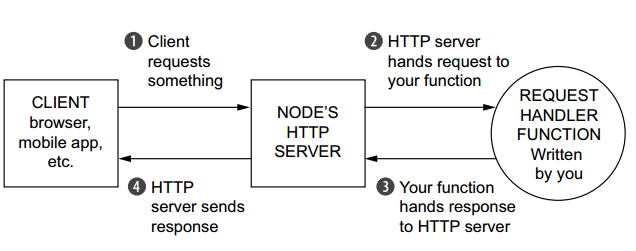
\includegraphics[height=6cm, width=0.7\textwidth, keepaspectratio]{nodemiddleware.png}
    \caption{\textit{NodeJs Middleware Yap�s�}}   
	\label{fig:middleware}
\end{figure}

Normal node yap�s�nda middleware yap�s� �ekil \ref{fig:middleware}'deki gibi i�lemektedir. Client istek yapar. Node http server bu iste�i yazd���m�z handler function yap�s�na iletir. Handler i�erisinde istek i�lenir ve http server'a tekrar yollan�r.	

Express kullan�rken middleware fonksiyonlar�n� kendimiz yazabiliriz veya haz�rda bulunan geli�tiriciler taraf�ndan yaz�l�m�� a��k kaynakl� module yap�lar�n� kullanabiliriz. A�a��daki yap� express middleware yap�s�n� g�stermektedir.


\begin{figure}[H] \centering
    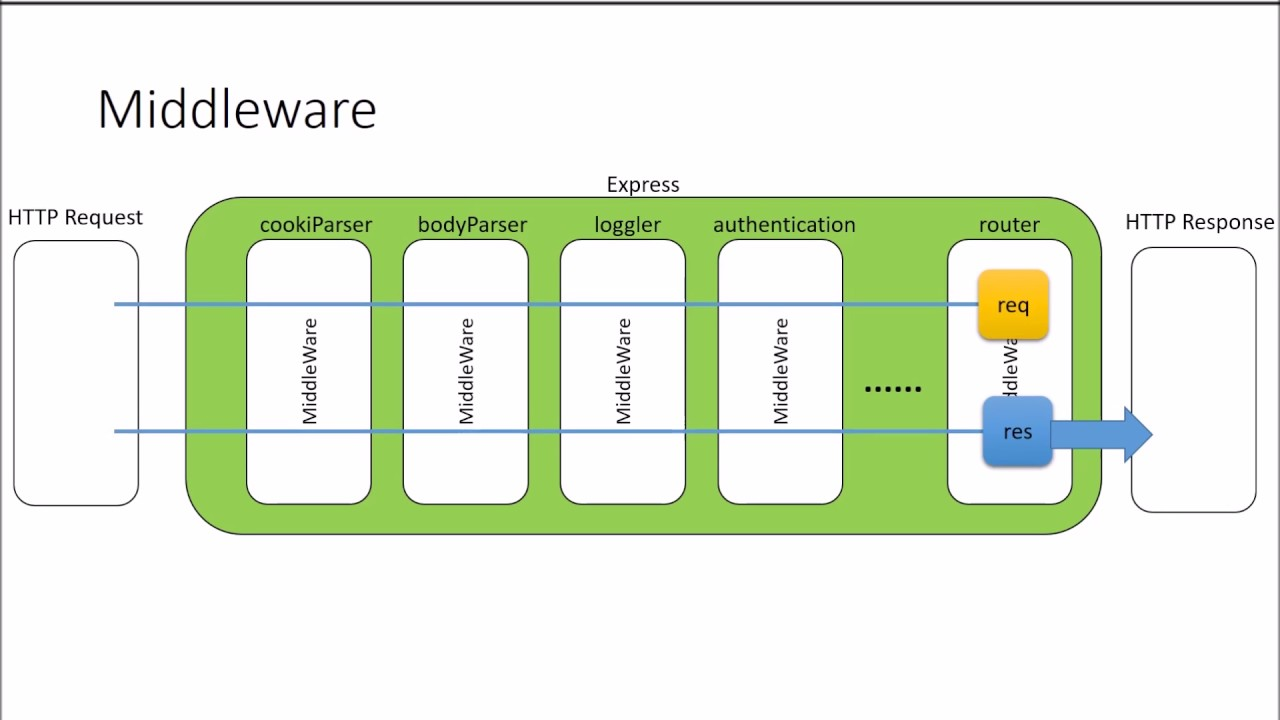
\includegraphics[height=6cm, width=0.7\textwidth, keepaspectratio]{expressmiddleware.jpg}
    \caption{\textit{ExpressJS Middleware Yap�s�}}
    \label{fig:expressmiddleware}
\end{figure}

ExpressJs Middleware yap�s�nda ise �ekil \ref{fig:expressmiddleware}'de g�sterildi�i gibi node http server �zerinden giden istekler stack yap�s�nda toplan�r. Stack yap�s� i�erisinde istek middleware fonksiyonlar�n� teker teker i�leyip sonunda response olarak http server'a kullan�c� iste�inin cevab�n� d�nd�r�r. Stack a�amas�nda middleware yap�lar� i�lenirken herhangi bir hata olu�tu�u durumda i�lem s�ras� kesilip hata middleware yap�s�na ge�ilmektedir. K�saca �zetlersek express frameworkte gelen istek stack yap�s� �zerinden yukar�dan a�a��ya do�ru t�m middleware i�lemlerinden ge�er.

Middleware fonksiyonlar� 3 parametre almaktad�r. Request ve response s�rekli bulunmal�d�r. Bunlar: function logger(request,response, next). Hata middleware yap�s� ise 4 parametre al�r. err, request, response, next 

�rnek verecek olursak; logger yaparken, console.log ile basit bir logger yap�s� yapar�z. E�er logger i�lemini ger�ekle�tirmek i�in haz�rlanm�� "morgan" ad� verilen module yap�s�n� kullan�rsak i�lemimizi k�salt�r�z. Sonu�ta tekerle�i yeniden icat etmemize gerek yok haz�r geli�tirilmi� mod�lleri kullan�p yapaca��m�z i�e odaklanmak daha mant�kl�d�r.

Express.js, middleware yap�s�n� kendi sitesinde basit�e anlatm��.�ekil \ref{fig:ornekExpress}'i k�saca �zetleyecek olursak. �nceden y�klenmi�(npm install express -save) express modul�n� ekliyor ve app de�i�kenine express uygulamas�n� tan�ml�yor.

\begin{figure}[H] \centering
    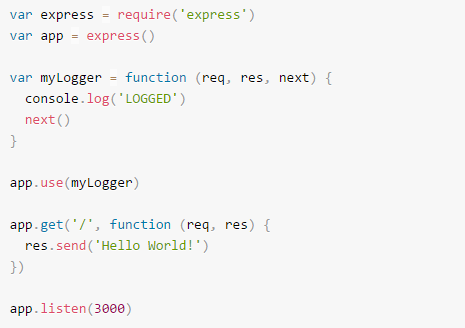
\includegraphics[height=6cm, width=0.8\textwidth, keepaspectratio]{ekran-alc4b1ntc4b1sc4b1.png}
    \caption{\textit{Express.js Kullan�m�}}
  	 \label{fig:ornekExpress}
\end{figure}

 Mylogger ile basit�e log yap�s� olu�turup next() metodu ile bir sonraki yap�y� �a��r�yor. app.use(myLogger) ile stack yap�s�na ekleme i�lemi yap�l�yor. Ard�ndan routing i�lemi yap�larak "/" yani a��l��ta g�sterilecek ilk ekrana "hello world" yazd�r�yor.





\subsection{Uygulamada Kullan�lan Node Mod�lleri}
\subsubsection{Morgan}
	Uygulama i�erisindeki HTTP request (isteklerini) loglamak i�in kullan�lan bir mod�ld�r. Bu mod�lle uygulamam�za gelen istekleri izleyebiliriz. �al��ma mekan�zmas� middleware �eklindedir (di�er pek �ok mod�lde oldu�u gibi). Gelen request morgan �zerinden ge�erken loglan�r.
\subsubsection{Body-Parser}
Bu mod�l isminden de anla��laca�� �zere uygulam�za gelen request'lerin body'lerinin kullan�lmak �zere parse edilmesini (ayr��t�r�lmas�n�) sa�lamaktad�r.
JSON, Text, Raw ve URL-enceded-form body'lerini parse edebilmekte, multipart request'leri ise parse ede\textbf{me}mektedir.

\subsubsection{Nodemon}
Front-end d�nyas�nda zaten �ok s�k kullan�lan bu teknolojinin, Back-end taraf�ndaki g�zel bir temsilcisidir. NodeJS ile uygulamalar geli�tirirken ayn� di�er backend teknolojilerinde oldu�u gibi kodlar�n �zerinde de�i�iklik yapt���m�zda sunumuzu tekrardan �al��t�rmam�z gerekiyor. \textbf{Nodemon} �al��ma ortam�m�zda dosyalar� s�rekli izleyerek dosyalardaki de�i�iklik durumunda Node sunucusunu yeniden ba�latmakta b�ylede yapt���m�z de�i�ikli�i hemen test edebilmemizi sa�lamaktad�r. 

\subsubsection{Lodash}
Lodash'� pek �o�umuz biliyoruz asl�nda. Front-end uygulamalar�n�n bir �o�unda JavaScrpit kodlar�m�z�n pek �ok i�lemi bizim yerimize performansl� olarak yapan k�t�phanedir. Yap�m� a�amas�nda esinlenildi�i Undurscore k�t�phanesine ek, pek �ok fonksiyon ve performans �st�nl��� eklemi�tir. �zellikle diziler (array) ve nesneler (object) �st�ne e�ilse de stringler gibi di�er konularda da gayet iyi ��z�mler sunuyor.
\subsubsection{Cookie-Parser}
Request ile gelen Cookie'leri okumak ve denece�imiz response'a cookie set etmek i�in kullan�lan mod�ld�r. Uygulama seviyesinde middleware olarak eklenir. 
\subsubsection{Passport}
NodeJS i�in en pop�ler \textbf{Authentication} mod�l�d�r. Kullan�c�lar�n kullan�c� ad� �ifreleri veya \textbf{OAuth} (Open Protocol) ile 3. parti (Facebook, Twitter, Google) hesaplar� ile authentication yapmas�n� sa�lamaktad�r. Authentication i�lemleri uygulaman�n ak�� �emas�n� ve davran��lar�n� de�i�tirebilecek bir yap�d�r. 
Dolay�s�yla Passport'u, Log gibi yerel olarak sadece uygulaman�n belli bir yerine eklenebilecek bir middleware yerine uygulama genelinde kullanabilece�imiz bir yap� olarak d���nebiliriz.

\subsubsection{dotenv}

Dotenv, ortam de�i�kenlerini bir .env dosyas�ndan process.env dosyas�na y�kleyen s�f�r ba��ml�l�k bir mod�ld�r. Yap�land�rmay� koddan ayr� bir ortamda saklamak i�in The Twelve-Factor App metodolojisine dayan�r.

\subsubsection{Mongoose}
MongoDB ile Node uygulamalar�n� yapabilmemiz i�in kullanaca��m�z mod�l�n ismi Mongoose'dur.
NodeJS d�nyas�nda olduk�a �nl� olan bu mod�l yakla��k 8.500 y�ld�za sahiptir. Bir�ok back-end teknolojisinde Relational veritabanlar� i�in \textbf{ORM} olarak tan�mlanan Object Relational Mapping'in Mongo taraf�ndaki kar��l��� olarak d���n�lebilir.

\subsubsection{PM2 Mod�l�}

Geli�tirmenizi tamamlad�n�z ama �retim ortam�nda uygulaman�z� �al��t�rman�z ve izlemeniz gerekiyor. ��te PM2 burada devreye giriyor ve size hatalar� log'lama, uygulaman�z �ld���nde tekrar �al��t�rma, kulland��� kaynaklar� izleme gibi imkanlar sunuyor.
PM2 uygulama process'lerinin s�reklili�ini sa�lamak i�in kullan�lan process manager'dir.

\subsection{Express Generator}
Express Generator projesiyle uygulaman�n ilk aya�a kalkmas� esnas�nda ihtiyac�n�z olacak yap� ve minik kod bloklar� eklenmi� �ekilde size bir iskelet sunuyor. B�ylece bu iskeleti olu�turmak i�in harcayaca��n�z zaman da size kal�yor.

�ncelikle \textbf{Express generator} isimli paketimizi kuruyoruz.
\begin{verbatim}
npm install express-generator -g
\end{verbatim}

Sonras�nda geli�tirece�miz uygulaman�n ismiyle 

\begin{verbatim}
express mustafaApp
\end{verbatim}

yazmam�z yeterli, Express-generator bizim i�in uygulamay� olu�turacakt�r.


\subsection{MongoDB}
MongoDB, ilk yay�nland��� 2009'dan bu yana sadece NodeJS de�il pek �ok back-end teknolojisi ile bir arada kullan�lan veritaban� ��z�m�d�r.
MongoDB'ye ge�meden �nce biraz geleneksel ili�kisel veritaban� mimarilerini d���nelim. Bir�ok tablonun oldu�u ve bu tablolar�n i�erisine gelecek verilerin \textbf{absolute} (kesin) bir �ekilde belirlendi�i, sonras�nda veritaban�n�n verileri al�rken de bu farkl� tablolar aras�nda ili�kiler kurularak verilerin al�nd���n� g�r�yoruz. 
�rnek olarak bir E-Ticaret sitesi d���nelim ve bu web uygulamas�n�n back-end taraf�ndan geleneksel veritaban� sistemleri ile yap�lm�� olsun. Bir sat�n alma olay�ndan sonra kullan�n�n ad�n� ve �r�nlerini ekrana yazd�raca��z. 
Bunun i�in minimum iki tabloya ihtiyac�m�z olacak. 
��yle ki;
\begin{enumerate}
\item Kullan�c�n�n t�m bilgilerini i�inde bar�nd�ran kullan�c� tablosu (isim, ya�, telefon, m��teri numaras� vs.
\item Ve sipari� detaylar�n� i�inde bar�nd�ran Order tablosu (Sipari� numaras�, sipari� saati, m��teri numaras� vs
\end{enumerate}

Yukar�daki �rnekte \textbf{User} tablosundan m��teri numaras� �zerinden ili�ki kurdu�umuz \textbf{Order} tablosundan verileri �ekebiliyoruz. Bu durumda iki tablo aras�ndaki ili�kiyi \textbf{customer\_id} isimli yani m��teri numaran�z� tutan \textbf{foreign key} ile sa�lad���m�z� varsayal�m. Bu basit i�lemde iki tablodan verileri ald�k. Peki listeleyece�imiz verilerde sat�n al�nan �r�nlerde olsayd�? Bu durumda yine database'in yap�s�na g�re en az 1 tabloya daha ihtiyac�m�z olacakt�.
Geleneksel mimaride i�ler bazen karma��kl�k durumuna g�re bir�ok tablo girdi�i i�in zorla�abiliyor. Bu durumda y�llar i�erisinde \textbf{NoSQL} olarak tan�mlanan bu geleneksel yakla��mdan ayr�lm�� ��z�mler ortaya ��kt�. \textbf{MongoDb}'de belkide bunlar�n en pop�leridir.
\textbf{NoSQL} sistemler ile verilerimizi anahtar de�er, \textbf{document oriented} gibi farkl� �ekillerden SQL'in kat� yap�s�na ba�l� kalmadan saklayabiliriz.

\textbf{MongoDB'nin �zellikleri �u �ekildedir}
\begin{enumerate}
\item �l�eklenebilirdir (Scalable). Veri boyutu artt��� durumlarda veya performans s�k�nt�s� ya�ad���m�z durumlarda makine ekleyebiliriz
\item Veriler document (belge) bi�iminde saklan�r. Burada JSON verilerini kullanabiliriz
\item Veriler JSON �eklinde sakland��� i�in gelen veri yap�s� de�i�se bile kaydetme i�leminde s�k�nt� ya�anmaz.
\item Verilerin birden fazla kopyas� saklanabilir ve veri kayb� ya�anmaz (Replication)
\item Veriler �zerinde index olu�turarak verilere h�zl� bir bi�imde ula�abiliriz
\end{enumerate}

\subsection{Redis}
	Redis, data structure'lar�m�z� saklamak i�in kulland���m�z bir teknolojidir. Redis in memory olarak �al���r, yani verileri bellekte tutmakta ve bu durum onu performans anlam�nda �ok �ne ��karmaktad�r. Kullan�m alanlar�n� inceledi�imizde �ok fazla data'n�n akt��� ve performans beklentisi gerektiren i�ler oldu�unu da g�r�yoruz. Session, Log vs...
\\
	Temel yap�s� <Key,Value> �eklinde olan Redis verileri String, Hash, Set, Sorted Set ve S�ral� List �eklinde tutar.
	
	\textbf{Avantajlar�}
	\begin{enumerate}
	\item CPU kullan�m�n� azalt�r.
	\item Performans art��� sa�lar.
	\item IO i�lemini azalt�r.
	\item Veriye ula��m� en basite indirir.
	\item A��k kaynak kodlu olmas� b�y�k bir avantaj.
	\item Bir�ok pop�ler yaz�l�m dilini desteklemektedir.
	\item Komutlar� kolay ve d�k�mante edilmi�tir.
	\item Bir�ok veri t�r�n� desteklemektedir.
	\item Senkron �al��maktad�r.
	\item Cluster Sharing, Sentinel, Replication gibi bir�ok enterprise �zelliklere sahiptir.
	\end{enumerate}

\textbf{Dezavantajlar�}

	\begin{enumerate}
	\item	Veri boyutu ile do�ru orant�l� olarak RAM ihtiyac�n�z artar.
	\item �li�kisel veritabanlar�nda oldu�u gibi karma��k sorgular� desteklemez.
	\item Join Mant��� yoktur.
	\item Transaction deste�i yoktur.
	\item Veri g�venli�i i�in bir kontrol mekanizmas� yoktur.
	\end{enumerate}
	
	
	\subsection{Socket.IO}
	Ger�ek zamanl� bir uygulama dendi�inde akla sunucudaki bir de�i�ikli�in an�nda istemci taraf�nda, istemci taraf�ndaki bir de�i�ikli�in an�nda sunucu taraf�nda de�i�ikli�e sahip olmas� olarak �zetleyebiliriz. 
	Son zamanlarda Web uygulamalar�nda pop�lerli�i ve kullan�m alan� giderek artsa da (Sosyal medya uygulamalar�ndaki chat implementasyonlar� gibi) asl�nda neredeyse internetin hayat�m�za girdi�i ilk zamanlardan beri teknolojik yap�s�n� ne olursa olsun kullanmaktay�z(IRC, ICQ gibi).
	Ancak zaman i�erisinde kullan�c� taraf�nda pratikte kullan�m� de�i�mese de altyap� olarak farkl�la�t���n� s�yleyebiliriz.
	�ncelikle Polling y�ntemiyle ba�layal�m.
	D�viz kular�n�n canl� olarak g�sterildi�i bir web sayfaas� yapt���m�z� d���nelim. Bu web sayfas� i�erisindeki rakamlar�n s�rekli olarak sunu taraf�nda g�ncellendi�ini varsayal�m. clilent taraf�nda sunucuya belli aral�klarla AJAX istek g�nderiyoruz. E�er de�i�iklik varsa View'imizi yeni datalarla g�ncelliyoruz.
	Ancak \textbf{Polling} y�nteminin �e�itli dezavantajalar� var.
	Tek y�nl� �al���yor. sunucudaki de�i�ikli�i sunucuya sormadan ��renemiyoruz. S�rekli olarak kontrol ama�l� sunucuya request gitti�i i�in fazladan sistem ve veriyolu kayna�� harcan�yor.
	Peki �imdi altyap�y� nas�l sa�l�yoruz?
	G�n�m�zde t�m modern browser'larda W3C taraf�ndan standart hale getirilmi� bir teknoloji olan Websocket protokol� kullan�lmaktad�r.
	Bu teknoloji Two way commutication sa�lar. Yani sunucudaki bir de�i�iklik istemci taraf�na, istemci taraf�ndaki bir de�i�iklik sunucu taraf�na \textbf{PUSH} yap�larak iletilir.
	Veirlerin Push ile akmas�, yani bir taraf�n di�er tarafa g�nclleme var m� diye sormadan e�er g�ncelleme varsa direkt olarak datalarla bildirmesi sistem kayna�� ve veriyolu anlma�nda avantaj sa�lamaktad�r. 
	Do�al olarak Polling metoduna g�re performans olarak h�zl�d�r (full dublex communication).
	
	\textbf{Websocket ile Socket.io aras�nda nas�l bir ili�ki var?}
	Websocket'in bu kadar geli�mi� bir yap�s� olmas�na ra�men direkt olarak kullanman�n baz� sak�ncalar� var. Bunlardan biri HTML5 standard� oldu�u i�in implementasyonunun sadece modern browser'lara yap�l�yor olmas�. 
	Geli�tirdi�imiz uygulamalar�n t�m kullan�c�lar taraf�ndan kullan�lmas�n� istiyorsak, Websocket kulland���m�zda eski taray�c�ya sahip kullan�clar kullanamayacakt�r.
	Socket.io, asl�nda Websocket �zerinde �al��an bir teknolojidir. Geli�tirici ile Websocket aras�nda Abstraction sa�layarak e�er kulland��� taray�c� Websocket desteklemiyorsa alternatif y�ntem �zerinden yine Real time haberle�meyi sa�layabilmektedir.
	Socket.io, client taraf�n�n socket ba�lant�s�n� a�mak istedi�i ilk request'te Websocket kullan�p kullanamayaca��n� kontrol ederek server ile ba�lant�s�n� configure etmektedir.
	Socket.io ile hem yap�sal hem de sonradan olu�turaca��m�z custom event'leri g�nderip alabiliyoruz.
	
	\subsection{AngularJS}
	
	AngularJS, dinamik web uygulamalar� i�in yap�sal bir frameworkt�r. HTML'i �ablon dili olarak kullanman�z� sa�lar ve uygulaman�n bile�enlerini a��k bir �ekilde ifade etmek i�in HTML s�zdizimini geni�letmenize izin verir. Angular'�n veri ba�lama ve ba��ml�l�k enjeksiyonu, aksi takdirde yazmak zorunda kalaca��n�z kodun �o�unu ortadan kald�r�r. Hepsi taray�c�da olur ve herhangi bir sunucu teknolojisi ile ideal bir ortakl�k yapar.
	\\\\
	
	\textbf{AngularJS �zellikleri}
	\begin{enumerate}
	\item AngularJS, Rich �nternet Uygulamas� (RIA) olu�turmak i�in g��l� bir JavaScript tabanl� geli�tirme �er�evesidir (framework).
	\item AngularJS, temiz bir MVC (Model View Controller) y�ntemiyle istemci taraf� uygulamas� (JavaScript kullanarak) yazmak i�in geli�tiriciler sa�lar.
	\item AngularJS ile yaz�lm�� uygulama �apraz (Cross) taray�c� uyumludur.
	\item AngularJS otomatik olarak her taray�c� i�in uygun JavaScript kodunu i�ler.
	\item AngularJS a��k kaynak kodlu, tamamen �cretsiz ve d�nyadaki binlerce geli�tirici taraf�ndan kullan�lmaktad�r. Apache Lisans� s�r�m 2.0 kapsam�nda lisanslanm��t�r.
	\item Genel olarak, AngularJS, bak�m� kolay bir �ekilde tutarak b�y�k �l�ekli ve y�ksek performansl� bir web uygulamas� olu�turmak i�in bir �er�evedir.
	\end{enumerate}

\textbf{AngularJS Temel �zellikleri}

\textbf{Veri ba�lama} - Model ve g�r�n�m bile�enleri aras�nda otomatik olarak veri senkronizasyonu.
\\\textbf{Kapsam} - Bunlar modele referans nesneleri. Denetleyici ve g�r�nt� aras�nda tutkal gibi davran�rlar.
\\\textbf{Denetleyici} - Bunlar belirli bir kapsama ba�l� olan JavaScript i�levleridir.
\\\textbf{Hizmetler} - AngularJS, XMLHttpRequests olu�turmak i�in \$ https: gibi �e�itli yerle�ik hizmetler ile birlikte gelir. Bunlar, yaln�zca bir kez uygulamada �rneklendirilen tek nesnelerdir.
\\\textbf{Filtreler} - Bunlar, bir dizideki ��elerin alt k�mesini se�er ve yeni bir dizi d�nd�r�r.
\\\textbf{Y�nergeler} - Y�nergeler, DOM ��elerindeki i�aretleyicidir (��eler, �zellikler, css ve daha fazlas� gibi). Bunlar, yeni ve �zel widget'lar olarak g�rev yapan �zel HTML etiketleri olu�turmak i�in kullan�labilir. AngularJS yerle�ik y�nergelere sahiptir (ngBind, ngModel ...)
\\\textbf{�ablonlar} - Bunlar, denetleyici ve modelden gelen bilgi i�eren i�lenmi� g�r�n�md�r. Bunlar, tek bir dosya (index.html gibi) veya "partials" kullanarak bir sayfada birden fazla g�r�n�m olabilir.
\\\textbf{Y�nlendirme} - G�r�� de�i�tirme kavram�.
\\\textbf{Model G�r�n�m� } - MVC, bir uygulamay� farkl� k�s�mlara (Model, G�r�n�m ve Denetleyici olarak adland�r�l�r) b�lmek i�in bir desen kal�b�d�r ve bunlar�n her biri farkl� sorumluluklara sahiptir. AngularJS MVC'yi geleneksel anlamda uygulam�yor, aksine MVVM'ye (Model-View-ViewModel) daha yak�nd�r. A��sal JS tak�m�, mizahi bir �ekilde Model G�r�n�m� olarak bahsetmektedir.
\\\textbf{Derin Ba�lant�} - Derin ba�lant�, URL'de yer alan uygulama durumunu kodlayarak yer imi eklemenizi sa�lar. Uygulama daha sonra URL'den ayn� duruma geri y�klenebilir.
\\\textbf{Ba��ml�l�k Enjeksiyonu} - AngularJS, uygulaman�n geli�tirilmesini, anla��lmas�n� ve test edilmesini kolayla�t�rarak geli�tiriciye yard�mc� olan yerle�ik ba��ml�l�k enjeksiyonu alt sistemine sahiptir.
	
	\textbf{AngularJS Avantajlar�}
	
	\begin{enumerate}
	\item AngularJS, Tek Sayfa Uygulamas�'n� �ok temiz ve bak�ml� bir �ekilde yaratma olana�� sa�lar.
	\item AngularJS, HTML'ye veri ba�lama yetene�i sa�lar ve b�ylece kullan�c�ya zengin ve duyarl� bir deneyim kazand�r�r
	\item AngularJS kodu birim test edilebilir.
	\item AngularJS ile geli�tirici daha az kod yazar ve daha fazla i�levsellik elde eder.
	\item AngularJS'de, g�r�n�mler saf html sayfalard�r ve JavaScript ile yaz�lm�� kontrol�rler i�lemlerini yapar.
	\end{enumerate}
	
	\newpage
	\section{Projeyi Canl�ya Alma Etme}
	Bu b�l�mde yap�lan projeyi nas�l canl�ya al�r�z, canl�ya alma i�lemleri yap�l�rken neler yap�lmal�d�r, hangi plaform bizim projemiz i�in daha do�ru bir yakla��m olacakt�r ve Git, github nedir projeler i�in neden �nemlidir bu konular �zerinde durulacakt�r.
\subsection{Git nedir?}
	��phesiz son  y�llardaki en pop�ler versiyon kontrol sistemi Git'dir. Projeler geli�tirirken ister tek ister ekip olarak �al��al�m, kodlar�m�z�n sa�l�kl� bir �ekilde tutulmas�, s�r�mlerin y�netilmesi i�in en �nemli g�rev Git'e d��mektedir.
	
	Genel olarak di�er \textbf{VCS} (Versiyon Kontrol Sistemi)'e g�re avantajlar� a�a��daki gibi s�ralayabiliriz. 
	\begin{enumerate}
	\item Da��t�k sistemli olmalar�ndan �t�r� ge�mi�te \textbf{SVN}(Subversion) ile ya�ad���m�z kod kayb� gibi pek �ok problemin �n�ne ge�mektedir. Sunucunun ��kmes� art�k eskisi kadar dert de�il. ��nk� herkeste t�m history'i i�eren local bir kopyas� var.
	\item Art�k ya�am alanlar�m�z�n her noktas�nda internet olsa da projelerimizde git kullan�yorsak projemizin localde tutuldu�u i�in internet ba�lant�s�na ihtiya� yoktur.
	\item H�zl�d�r. Y�zlerce MB'l�k projeleri bile olduk�a rahat bu sisteme dahil edebilirsiniz. 
	\item Bir�ok geli�tiricinin bulundu�u projelerde merge i�lemi sanc�l�d�r. Gir di�er VCS'lere nazaran merge i�leminde daha ba�ar�l�.
	\item Basit i�lemleri ��renmesi kolay ama sonraki a�amada ileri seviyeye ��kmak o kadar kolay de�il s�rf Git'in ak��� i�in bir�ok pattern geli�tirilmi� durumda.
	\item Braching mekanizmas� olduk�a geli�mi�tir.
	\item Github gibi a��k kaynak i�in tekel olan bir uygulamada kullan�l�yor.
\end{enumerate}	

\subsection{Sunucu Se�imi}
Geli�tirdi�imiz projeleri son kullan�c�ya iletmek i�in sunucu �zerinden yay�nlamam�z gerekiyor. �nternetin ilk zamanlar�nda bu sunucu �zerinde bir shared hosting kiralay�p kullan�c�lara sunma y�n�ndeydi. Shared hosting'de onlarca farkl� uygulama ayn� anda isminden de belli oldu�u gibi 1 shared environment'de �al��maktad�r. Bu da beraberinde her ne kadar olduk�a maliyetsiz bir ��z�m y�ntemi olsa da performans ve g�venlik sorunlar�n� do�urmaktad�r. Godaddy gibi bir�ok firma bu konudaki �r�nlerini sunmaya devam etmektedir.
	Ancak bu nokada art�k internet kullanan ki�i say�s�n�n y�llar i�erisinde artmas� ve buna ba�l� olarak cloud mimarilerinin geli�mesi production'daki �r�nlerin daha sa�lam ve scale edilebilir sistemler �zerinde yay�nlanmas�n� beraberinde getirdi.
	�u anda en pop�ler iki mimari olan \textbf{Platform as a Service} (PaaS) ve \textbf{Infrastructure as a Service} (IaaS) kavramlar�n� inceleyelim.
	
	\textbf{Paas:} Sundu�u yap�yla geli�ticileri sistem bilgisine sahip olmasalar bile kendi yap�lar� �zerinde �al��t�rmay� varsaymaktad�r. ��erisinde bar�nd�rd��� pek �ok servisle geli�tirme s�re�lerine katk� sa�lamaktad�rlar. �unu kabul etmemiz gerekir ki sistem s�re�leri, sistemin kaynaklar�n�n y�netimi en az yaz�l�m kadar geli�tiriciyi zorlamaktad�r.
	Nispeten daha kolay kullan�m a��s�ndan Paas ��z�mler Iaas sistemlerden �ne ��karken, g�venlik ve esneklik ile shared hosting'lerden �ok hada iyi konumdad�r.
	Paas hizmeti veren en �nemli firmalar a�a��daki gibidir.
	
	Heroku, Digital Ocean, EngineYard, OpenShift.
	
	\textbf{IaaS:} Buluut bili�imiz en \textbf{low level} hizmeti olarak ifade edebiliriz. Hizmeti sunan firma taraf�ndan ki�iye a��lacak sanal sunucunun y�netimini (ekstra hizmetlerde sunabilmekte) geli�tirici taraf�na b�rakmaktad�r. IaaS tipi yap�lar� kullanabilmek i�in sistem taraf�nda bilginiz olmas� gerekiyor. Bu hizmeti ald���m�z firma sunucu �zerindeki hemen hemen her�eyin bizim taraf�m�zdan yap�labilece�ini belirtiyor. Bunun ��kt�s� olarak da olduk�a esnek, scale edebilen sistemler geli�tirebiliyoruz. IaaS hizmeti veren en �nemli firmalar AWS, Azure ve Rackspace'dir.
	Iaas ve Paas aras�dnaki genel farklar� inceledikten sonra deploy i�lemini ilk denedi�im ama redis yap�land�rmas�n� yapamad���m i�in yar�da kalan Heroku'dan size bahsetmek istiyorum.
	
	\subsubsection{Heroku}
	Heroku destek verdi�i bir�ok dil ve kullan�m kolayl��� ile �ne ��kan \textbf{Platform as a Service} tipinde bir firmad�r. Genelde k���k ve orta �l�ekli projeler ya da prototip uygulamalar i�in tercih edilmektedir. En b�y�k �zlli�inin kolay kullan�m� ve h�zl� deploy yapabilme imkan� tan�mas� oldu�unu tekrar hat�rlatay�m. 
	AWS gibi sistemler maalesef her geli�tiriciye hitap etmeyebiliyor. ��nk� bu yap�lar� kullanabilmek i�in en az�ndan orta �l�ekli bir sistem bilgisine ihtiya� bulunmaktad�r. Bunun yan�nda Digital Ocean gibi ara ��z�mlerde bulunmaktad�r. Bunun yan�nda \textbf{Heroku} e�er k�sa ve orta vadede h�zl� scale etmeniz gereken bir projenize varsa maliyet olarak biraz fazla y�k getirece�ini belirteyim.
	�imdi sizlere kullanm�� oldu�um ve redis yap�land�rmam dahil herhangi bir problem ya�amad���m Digital Ocean'dan bahsetmek istiyorum.
	\subsubsection{DigitalOcean nedir? Ne yapar?}
	DigitalOcean, bulut tabanl� altyap� sa�lay�c�s� olarak kendini konumland�ran, geli�tirme, s�r�m kontrol� ve test ortamlar� gibi bir �ok ihtiyaca cevap veren d�nyan�n en b�y�k bulut sunucu sa�lay�c�lar�ndan biri. Tabi, detaylara bak�ld���nda �ekil \ref{fig:digitalOcean}'deki markalar�n farkl� sorunlara odakland�klar� da a�ikar.
	
\begin{figure}[H] \centering
    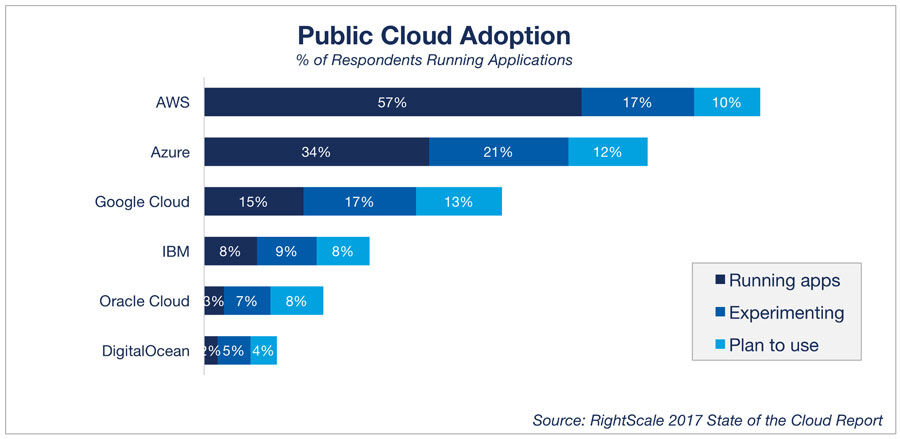
\includegraphics[height=6cm, width=0.8\textwidth, keepaspectratio]{digitalocean-1.jpg}
    \caption{\textit{Genel Bulut Kullan�m�}}
    \label{fig:digitalOcean}
\end{figure}
	
	 �rne�in Amazon ile kesi�en noktalar (Lightsail) d���nda resmin tamam�na bakt���m�zda Amazon rekabetinin �o�unlukla Google AppEngine ve Microsoft Azure taraf�nda yo�unluk kazand���n� g�rebiliriz.
	
	



\textbf{DigitalOcean geli�tiricilere neler sunuyor?}

\begin{enumerate}
\item Kullan�m Kolayl��� \\
\textbf{Droplet} ad� alt�nda ifade edilen bulut sunuculara Image yada app tercihi, kapasite ve b�lge se�iminizin ard�ndan saniyeler i�erisinde 1 dakikadan az bir s�rede sahip olabilir, olu�turdu�unuz dropletleri pratik bir �ekilde kontrol edebilirsiniz. Ayr�ca, API �zerinden de droplet kontrolleri ger�ekle�tirebilmektesiniz.
\item \textbf{SSD Disk} Verileriniz performans� y�ksek ve standart olarak sunulan SSD disklerde tutulmakta.
\item \textbf{�cretlendirme Avantaj�} Ayl�k minimumda \$5 (saatlik \$0.007)'dan ba�layan fiyatlarla kullan�ma ba�layabilirsiniz. Droplet pasif oldu�u durumlarda da veri bar�nd�rd��� i�in saatlik �cret i�lemeye devam ediyor. Image al�p droplet'i kald�rarak test kullan�mlar�n� �ok daha efektif bir fiyatland�rmayla s�rd�rebilirsiniz.
\item \textbf{Distro Se�imleri} Olu�turaca��n�z droplet i�in Ubuntu, CentOS, Debian, Fedora, CoreOS gibi bir linux da��t�mlar�n�n yan� s�ra FreeBSD de se�ebilirsiniz.
\item \textbf{Tek T�kla App Kurulumu} LAMP, LEMP, MEAN, Django, Ghost, WordPress ve Docker gibi tek t�klama ile pop�ler bir �ok uygulama kurulumunu h�zl�ca ger�ekle�tirebilirsiniz.
\item \textbf{Teknik Destek} Kar��la�abilece�iniz bir �ok soruna y�nelik olarak haz�rlanm�� olduk�a kullan��l� bir i�erik y���n�na sahipler. Ek olarak, i�erik dahilinde ula�amad���n�z ��z�mlere kom�nite �zerinden h�zl� bir �ekilde cevap alabilirsiniz. Hala ��z�ms�z kalm��san�z h�zl� d�n�� alabilece�iniz bir ticket olu�turabilirsiniz.
\end{enumerate}

\subsubsection{Droplet}
Kullan�m� kolay ve yeniden boyutland�r�labilir bulut sunucusudur (VPS).

\begin{enumerate}
\item Bir Linux da��t�m�n�, uygulamay� se�erek ya da �nceden olu�turdu�umuz snapshor ile Droplet olu�turabiliriz.
\item �htiyac�m�z olan kaynaklara dayal� bir Droplet boyutunu se�ip. Kontrol panelinden istedi�imiz zaman yeniden \textbf{dikey} (vertical) boyutland�rabiliriz. Dikey boyutland�rma mevcut Droplet'in (sunucu) \textbf{CPU, RAM} veya \textbf{Diskinin �l�eklendirmesi} (scalability) anlam�ndad�r. \textbf{Yatay} (Horizontal) �l�eklendirme ise; mevcut havuza daha fazla makine (VPS-Droplet) ekleyerek dinamik olarak �l�eklendirmektir.
\item Droplet'i d�nya �zerinde bulunan farkl� veri merkezlerinden (datacenter) birini se�erek olu�turabilirsiniz. Burda dikkat edilmesi gereken, baz� datacenter b�lgelerinin (region) neleri destekleyip desteklemedi�idir.
\end{enumerate}

\textbf{�zellikler:}
\begin{itemize}
\item \textbf{Cluster Deployment: }Olu�turdu�umuz her Droplet bir cluster (k�me)�yesidir.
\item \textbf{Resize: }�htiyac�n�za ba�l� olarak Droplet'lerimizin (Droplets) kaynaklar�n� dikey olarak �l�eklendirin.
\item \textbf{Yedekleme ve G�r�nt� Alma: }droplet olu�truma s�ras�nda otomatik yedeklemeleri (backup) etkinle�tirim veya istedi�iniz zaman anl�k g�r�nt� (snapshot) al�n.
\item \textbf{�zleme: }Droplet'lerimizin bant geni�li�i, disk ve CpU seviyelerini yak�ndan takip edin.
\item \textbf{User Data: }�lk kurulum s�ras�nda paketlerin y�klenmesini otomatikle�timek i�in �zel komut dosyalar� ekleyin.
\item \textbf{User Data: }�lk kurulum s�ras�nda paketlerin y�klenmesini otomatikle�tirmek i�in �zel komut dosyalr� ekleyin.
\item \textbf{40GbE: }40 Gigabit Ethernet (40GbE), Ethernet �er�evelerinin (frame) saniyede 40 gigabit'e (GbpS) kadar aktar�m�n� sa�layan bir standartt�r. 40GbE standard� yerel sunucu ba�lant�s� i�in tasarlanm��t�r; Daha sa�lam standart, 100 Gigabit Etherne (100GbE), �nternet omurgalar�na y�neliktir.
\textbf{KVM: }Geli�mi� a� performans� ve g�venli�i i�in kurumsal d�zeyde KVM.
\textbf{Droplet aras� haberle�me: }Dropletlerimiz birbiriyle private network olana�� ile haberle�ebilir.
\end{itemize}

\newpage
\section{Web Sitesinin G�r�nt�leri}
Bu b�l�mde yaz�lan projenin front-end g�r�n�m� payla��lacak olup, giri� sayfas� mesajla�ma sayfas� ve projeye do�rudan girmenizi saylayacak kare kodu payla��lacakt�r muhtemelen art�k o siteye eri�imizin olamayaca��n� da belirtmek isterim.
\subsection{Giri� Sayfas�}
Projemize ait giri� sayfas� �ekil \ref{fig: kullaniciSayfasi}'de g�r�nd��� gibidir.
\begin{figure}[H] \centering
    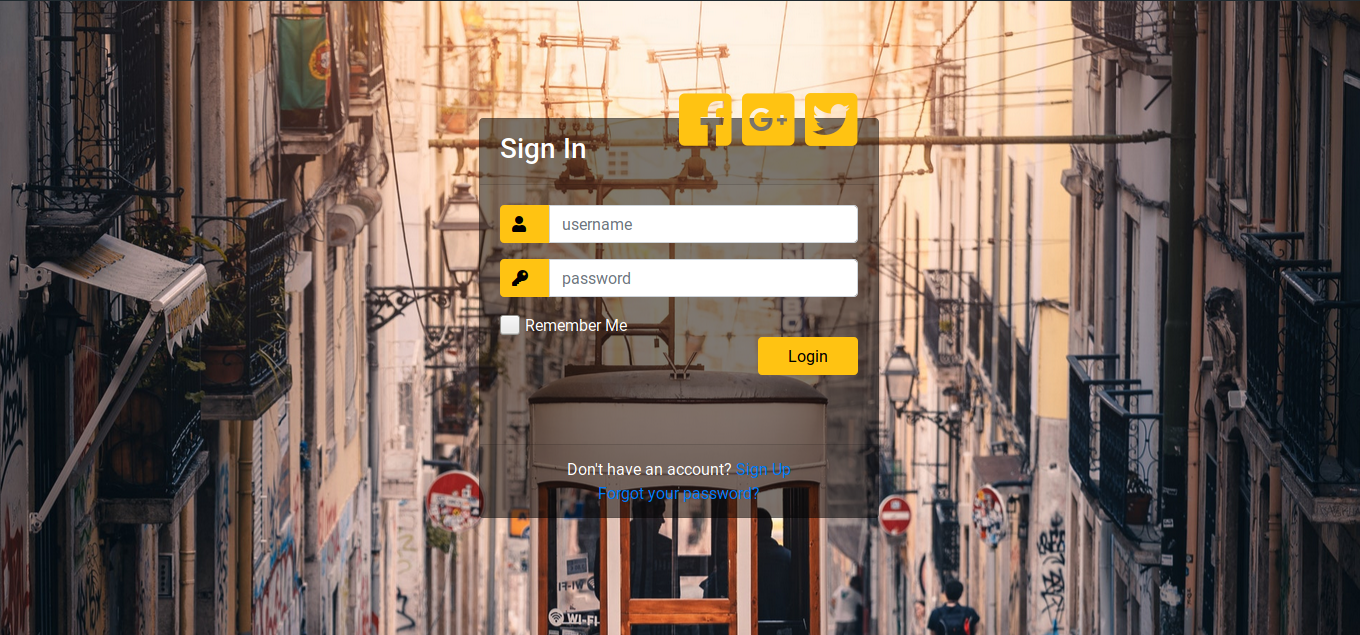
\includegraphics[height=6cm, width=0.8\textwidth, keepaspectratio]{anasayfa.png}
    \caption{\textit{Kullan�c� Giri� Sayfas�}}
    \label{fig: kullaniciSayfasi}
\end{figure}


\subsection{Mesajla�ma Sayfas�}
Projeye ait mesajla�ma sayfas� �ekil \ref{fig: mesajlasma}'deki gibidir.
\begin{figure}[H] \centering
    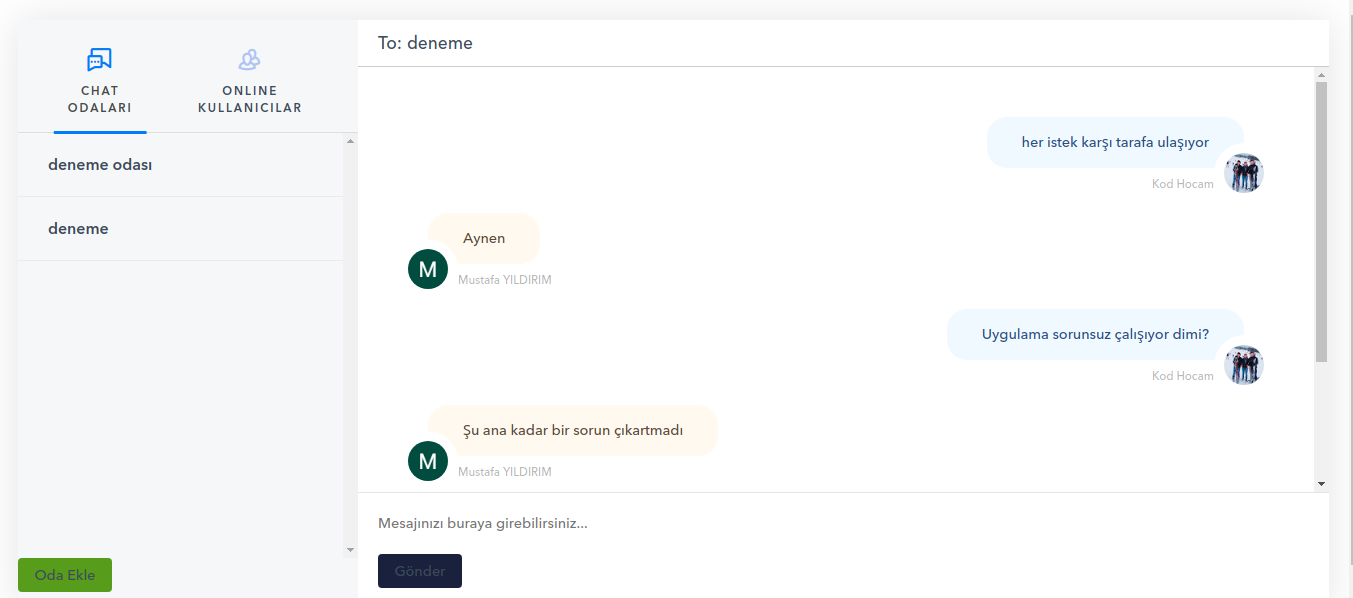
\includegraphics[height=6cm, width=0.8\textwidth, keepaspectratio]{main.png}
    \caption{\textit{Mesajla�ma Sayfas�}}
    \label{fig: mesajlasma}
\end{figure}

\subsection{Sitemi denemek ister misiniz?}
E�er sitemi denemek isterseniz �ekil \ref{fig: kareKod}'deki kare kodu taratarak ilgili sayfaya gidebilirsiniz.
 	\begin{figure}[H] \centering
    
\includegraphics[height=6cm, width=0.8\textwidth, keepaspectratio]{qrcode.png}
    \caption{\textit{Sayfay� a�acak olan karekodu}}
    \label{fig: kareKod}
\end{figure}

	
	
	
%\section{Uygulama A�amalar� ve Sistemin Geli�tirilmesi}

%\section{KULLANILAN BILESENLER}
	
	
%\section{ADI}

\section{SONU�LAR VE �NER�LER}

Yapm�� oldu�um uygulamada g�zlemlediklerime g�re �u anda t�m sistemler sadece node.js ve NoSql yap�lar� kullan�larak olu�turulmuyor olsalarda �n�m�zdeki 4 - 5 sene i�erisinde geleneksel format yava� bir �ekilde b�rak�larak yerine yenilik�i metodlar gelecek gibi g�r�n�yor. Uygulamay� Node.Js'le yazarken g�zlemlerime g�re php ile veya di�er geleneksel teknolojilerler uygulama yazarken �l�eklenebilirlik sorunu ile kar�� kar��ya kal�yoruz. Bu problemin �stesinden klasik (geleneksel) y�ntemlerle de gelebiliriz ama bu bizim i�in daha maliyetli bir yakla��m olur. Bunun yerine h�zl� �l�eklenebilir bir yap� olan Node.Js kullanmak daha mant�kl� ve maliyetsiz bir yakla��m olacakt�r. Bunlara ek olarak benim kulland���m yap�n�n daha g�zel bir �ekilde kullan�lm�� hali bulunmakta buna \textbf{MEAN} diyorlar.
Mongo, Express, Angular ve Node teknolojilerinin birle�mesiyle dinamik web uygulamar� yapmak i�in �retilen stack'leri anlatmak i�in kullan�lan bir terimdir. Mean.io adresinden geli�tirilmesi devam eden MEAN stack haricinde farkl� MEAN Stack implemantasyon bulunmaktad�r. 
MEAN stack kendisini bu �nl� 4 teknolojiyi bulu�turan bir Framework olarak tan�mlamaktad�r. Bu yap�n�n ortaya ��kmas�ndaki neden de yap�lan yap�lan back-end uygulamalar� daha modern bir �ekilde kullan�c�lar�n �n�ne getirme ihtiyac�d�r. Web uygulamar�nda view katman� JavaScript ve UX kavramlar�n�n geli�imi ile giderek farkl�la�maktad�r. ��te bu noktada MEAN yap�s� bize sa�lad��� back-end yap�land�rmas�n�n yan�nda Angular deste�i ile kolayl�k sa�lamaktad�r. K�saca bu uygulama i�in kulland���m teknolojiyi yapt���m ara�t�rmalardan yola ��karak en do�ru ve kesin sonu� olarak g�r�yorum. Server-client aras�nda s�rekli ve �ift y�nl� etkile�im olan uygulamalarda kullan�lmas�n� tavsiye ediyorum.
%\section{EKLER}

\renewcommand{\refname}{KAYNAKLAR}
\addcontentsline{toc}{section}{KAYNAKLAR}
\begin{thebibliography}{99}%kaynak ortam� olu�turmak i�in

\bibitem{k:1} CTAN,\url{https://www.codeinwp.com/blog/angular-vs-vue-vs-react/} [Ziyaret Tarihi: 25 Mart 2019]
\bibitem{k:2} CTAN,\url{https://gelecegiyazanlar.turkcell.com.tr/konu/web-programlama/egitim/301-javascript/javascript-nedir} [Ziyaret Tarihi: 29 Mart 2019]
\bibitem{k:4} CTAN,\url{https://www.mobilhanem.com/angular-dersleri-angular-nedir/} [Ziyaret Tarihi: 2 Nisan 2019]
\bibitem{k:3} CTAN,\url{https://kodcu.com/2013/04/nosql-kavrami-ve-mongodb/} [Ziyaret Tarihi: 12 May�s 2019]
\bibitem{k:5} CTAN,\url{https://nodejs.org/en/} [Ziyaret Tarihi: 14 Mart 2019]
\bibitem{k:6} CTAN,\url{https://angular.io/} [Ziyaret Tarihi: 15 Mart 2019]
\bibitem{k:7} CTAN,\url{https://expressjs.com/} [Ziyaret Tarihi: 12 May�s 2019]
\bibitem{k:8} CTAN,\url{https://redis.io/} [Ziyaret Tarihi: 12 May�s 2019]
\bibitem{k:9} CTAN,\url{https://www.mongodb.com/} [Ziyaret Tarihi: 12 May�s 2019]
\end{thebibliography}
\centerline{\textbf{�ZGE�M��}}
\addcontentsline{toc}{section}{�ZGE�M��}
\begin{table}[H]
{
\renewcommand{\arraystretch}{1.5}
\begin{tabular}{l@{\bf :}l}
\multicolumn{2}{l}{\underline{\bf K���SEL B�LG�LER}}\cr
\textbf{Ad� Soyad�}&  Mustafa YILDIRIM   \cr
\textbf{Uyru�u}&\; T�rk \cr
\textbf{Do�um Yeri ve Tarihi}&\;  �sk�dar 12.05.1997   \cr
\textbf{Adres}&\;      \cr
\multicolumn{1}{l}{}&      \cr
\textbf{Telefon}&\;  +905466678093   \cr
\textbf{e-mail}&\; musttafayildirim@gmail.com  \cr
\multicolumn{1}{l}{}&\cr
\multicolumn{2}{l}{\underline{\bf E��T�M DURUMU}}\cr
\textbf{Lisans ��renimi}&\; B�E� Bilgisayar M�hendisli�i B�l�m�\cr
\textbf{Bitirme Y�l�}&\;    \cr
\textbf{Lise}& \;  A.�.L  \cr
\multicolumn{1}{l}{}&\cr
\multicolumn{2}{l}{\underline{\bf �� DENEY�MLER�}}\cr
\textbf{Y�l}&\;     \cr
\textbf{Kurum}& \;    \cr
\textbf{Stajlar}&\;     \cr
\multicolumn{1}{l}{}&\cr
\multicolumn{2}{l}{\underline{\bf �LG� ALANLARI:}}\cr
\multicolumn{1}{l}{}&\cr
\multicolumn{2}{l}{\underline{\bf YABANCI D�LLER:}}\cr
\multicolumn{1}{l}{}&\cr
\multicolumn{2}{l}{\underline{\bf BEL�RTMEK �STED���N�Z D��ER �ZELL�KLER:}}
\end{tabular}}
\end{table}
\shorthandon{=}
\end{document}
%%%%%%%%%%%%%%%%%%%%%%%%%%%B�TT�%%%%%%%%%%%%%%%%%%%%%%%%%%%%%%%%%%%%%%%%%%%%%
